
\section{Differential Evolution}

DE is a population-based optimization algorithm, where operators for mutation, crossover and selection act to create a new population from an existing one such that eventually, through a series of iterations, the population will converge on to a globally optimal solution \cite{Poole3}. DE is suitable for problems with discontinues objectives, also with a problem having multiple local optima (multimodality). But are associated with slow convergence. Nearly 200 times more functional evaluations are required for Gradient-free methods as compared to gradient-based methods \cite{oleg}.

Differential Evolution (DE) is a parallel direct search method which utilizes NP
D-dimensional parameter vectors,
$$x_{i,G} \hspace{2mm} i = 1, 2, ... , NP$$
as a population for each generation G. NP does not change during the minimization
process. The initial vector population is chosen randomly and should cover the entire
parameter space. As a rule, it is assumed to follow a uniform probability distribution for
all random decisions unless otherwise stated. In case a preliminary solution is
available, the initial population might be generated by adding normally distributed
random deviations to the nominal solution $x_{nom,0}$. DE generates new parameter
vectors by adding the weighted difference between two population vectors to a
third vector. Let this operation be called \textit{mutation}.

The mutated vector’s parameters are then mixed with the parameters of another predetermined vector, the target vector, to yield the so-called \textit{trial vector}. Parameter mixing is often referred to as “\textit{crossover}” . If the trial vector yields a lower cost function value than the target vector, the trial vector replaces the target vector in the following generation. This last operation is called \textit{selection}. Each population vector has to serve once as the target vector so that NP competitions take place in one generation.\cite{storn}

The mathematical representation of the DE algorithm is explained here,
\begin{enumerate}
\item \underline{Initialization} : Here the initial population (N) is opted on random basis, which will be of size $d$-th dimension $(d\in\{1, \ldots, D\}))$ is given as: 
\begin{equation}
\textbf{x}_{n,g}^{d}=\textbf{L}^{d}+\operatorname{rand}(0,1)\left(\textbf{U}^{d}-\textbf{L}^{d}\right)
\label{initlize}
\end{equation}
where rand(0,1) is a uniformly distributed random number on the interval [0,1].

\item \underline{Mutation}: For each individual in population size, corresponding donor vector is generated by taking weighted difference between any two randomly selected vectors, and add it to third vector which is again selected randomly as shown. 
\begin{equation}
\mathbf{v}_{n}=\mathbf{x}_{r_{1}}(t)+F\left(\mathbf{x}_{r_{2}}(t)-\mathbf{x}_{r_{3}}(t)\right)
\label{normal_mutation}
\end{equation}
where, F is the scaling factor,and  \(r_{1}, r_{2}\) and \(r_{3}\) and \(r_{3}\) and \(r_{3}\) are uniformly distributed random integers on the interval \([1, N]\) such that \(r_{1} \neq r_{2} \neq r_{3} \neq n .\) The \(n\) -th donor vector using the DE/best/1 strategy is:
\begin{equation}
\mathbf{v}_{n}=\mathbf{x}_{b}(t)+F\left(\mathbf{x}_{r_{1}}(t)-\mathbf{x}_{r_{2}}(t)\right)
\label{best_mutation}
\end{equation}
$$
b=\underset{i \in\{1, \ldots, N\}}{\arg \min } f\left(\mathbf{x}_{i}\right)
$$
so $x_b$ is the best individual in the population. Also $r_1$ and $r_2$ are uniformly distributed random integers in the interval [1,N] such that \(r_{1} \neq r_{2} \neq b\) and \(r_{1} \neq r_{2} \neq n\). The better representation of mutation stage in 2-D design space is as shown below.
\begin{figure}[!ht]
    \centering
    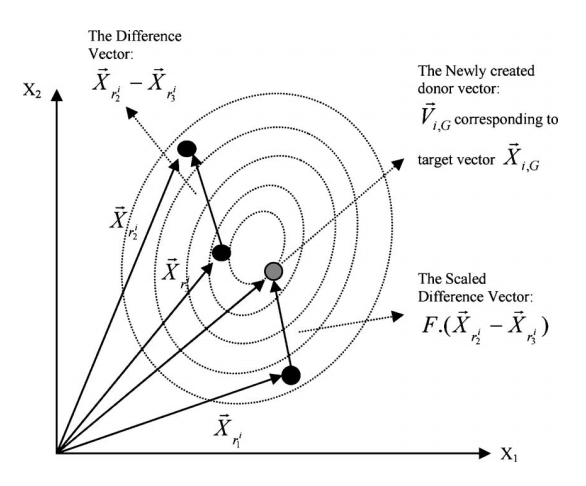
\includegraphics[scale = 0.5]{figures/mutation.png}
    \caption{2-D design space representing mutation stage\cite{storn}}
    \label{mutation}
\end{figure}

\item \underline{Cross-over} :This is the stage where elements from target vector and donor vectors are combined in specific order to get trial vector as shown. This stage is important because it increases the diversity in the population as shown,
\begin{figure}[!ht]
    \centering
    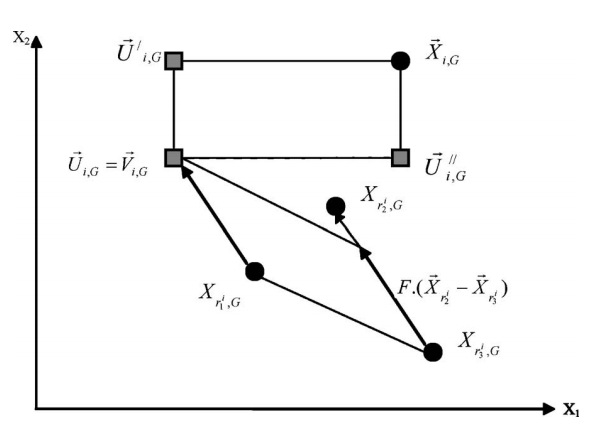
\includegraphics[scale = 0.5]{figures/crossover.png}
    \caption{Different possible trial vector formed due to Uniform/Binomial crossover between mutant vector and target vector in 2-D design space\cite{storn}}
    \label{crossover}
\end{figure}
\begin{equation}
\mathbf{u}_{n,g}=\left\{\begin{array}{ll}{\mathbf{v}_{n,g}} & {\text { if rand }(0,1) \leq C R \text { or } r_{n}=d} \\ {\mathbf{x}_{n,g}} & {\text { otherwise }}\end{array}\right.
\label{cross-over}
\end{equation}
where $r_n$ is the uniformly distributed random integer in the interval [1,D] and CR is the cross probability. CR = 0 implies there is no diversity, meaning the parent elements are not carried to next generation (iteration). On the other hand, CR = 1 implies all elements which are generated will be parents elements itself , so there is no evolution with iteration.

\item \underline{Selection} :The Trial vector and Target vector are compared with their function value, if the function is of minimization case, then the one with lesser function value is retained. On the other hand, if the function is of maximization case, the one with maximum function evaluation is retained.
\begin{equation}
\mathbf{x}_{n}(t+1)=\left\{\begin{array}{ll}{\mathbf{u}_{n}} & {\text { if } f\left(\mathbf{u}_{n}\right) \leq f\left(\mathbf{x}_{n}(t)\right)} \\ {\mathbf{x}_{n}(t)} & {\text { otherwise }}\end{array}\right.
\label{selection}
\end{equation}

\item \underline{Stopping condition}: Here the optimization can have one or multiple stopping conditions, like maximum number of function evaluation, epsilon value, etc. In the paper mentioned as above, author throughout the paper use the maximum number of function evaluation ($FEs_{max}$) as the stopping condition for all the algorithms.
\end{enumerate}
The Pseudo-code for the DE algorithm is shown below.
\begin{algorithm}[!ht]
\SetAlgoNoLine
 Randomly initialise individuals and calculate objective\\
 \While{\text { $FEs <FEs_{max}$ }}
 {
  \For{$n=1 \rightarrow N$}
  {
  Perform mutation: equation \ref{best_mutation}\\
  Perform binomial crossover: equation \ref{cross-over}\\
  Calculate objective and constraints of trial vector
  }
  \For{$n=1 \rightarrow N$}{
 Update $n$-th target vector: equation \ref{selection}
 }
 }
 \caption{DE algorithm}
 \label{DE algorithm}
\end{algorithm}
\section{DE Strategies}
In the DE algorithm, there are different variants for mutation stage. Some of the these are mentioned and explained here,\cite{chi}

\subsection{DE/rand/1}
In this method, the mutation stage is carried out by taking single pair of the weighted difference of vectors which are picked randomly from the previous generation and added to base vector, which is again picked randomly to form the target vector as shown.
\begin{equation}
    \mathbf{v}_{n, g}=\mathbf{x}_{r_{1}, g}+F.\left(\mathbf{x}_{r_{2}, g}-\mathbf{x}_{r_{3}, g}\right)
    \label{DE-rand-1}
\end{equation}

\subsection{DE/best/1}
This method work the same way as $DE/rand/1$, except that it generates the individual base vector $x_{b}$ as shown below,
\begin{equation}
    \mathbf{v}_{n, g}=\mathbf{x}_{b, g-1}+F.\left(\mathbf{x}_{r_{1}, g}-\mathbf{x}_{r_{2}, g}\right)
    \label{DE-best-1}
\end{equation}
where,
$$
b=\underset{i \in\{1, \ldots, N\}}{\arg \min } f\left(\mathbf{x}_{i, g-1}\right)
$$

\subsection{DE/best/2}
Here in this method, the perturbed vector  (mutation vector) will have two weighted ($F_1, F_2$) differences of vectors which are picked randomly from the population size \(N\) and added to base vector (best) \(x_b\) as shown.
\begin{equation}
  \mathbf{v}_{n, g}=\mathbf{x}_{b, g-1}
+F_{1}.\left(\mathbf{x}_{r_{1}, g}-\mathbf{x}_{r_{2}, g}\right)
+F_{2}.\left(\mathbf{x}_{r_{3}, g}-\mathbf{x}_{r_{4}, g}\right)
\label{DE-best-2}
\end{equation}
where,
$$
b=\underset{i \in\{1, \ldots, N\}}{\arg \min } f\left(\mathbf{x}_{i, g}\right)
$$


\subsection{DE/current to best/2}
In this method, one of the two weighted differences will take place between the best vector and the vector index for which perturbation is carried out, and the formula is as shown below, 
$$\mathbf{v}_{n}=\mathbf{x}_{b}(t)
+F_{1}\left(\mathbf{x}_{r_{1}}(t)-\mathbf{x}_{r_{2}}(t)\right)
+F_{2}\left(\mathbf{x}_{b}(t)-\mathbf{x}_{r_n}(t)\right)$$
where,
$$
b=\underset{i \in\{1, \ldots, N\}}{\arg \min } f\left(\mathbf{x}_{i}\right)
$$

\subsection{DE/rand/2}
In this method, there exist two weighted differences between randomly chosen population vectors, and all the vectors are randomly selected. 
$$\mathbf{v}_{n}=\mathbf{x}_{r_{1}}(t)
+F_{1}\left(\mathbf{x}_{r_{2}}(t)-\mathbf{x}_{r_{3}}(t)\right)
+F_{2}\left(\mathbf{x}_{r_{4}}(t)-\mathbf{x}_{r_{5}}(t)\right)$$
where, $r_1, r_2, r_3, r_4, r_5 \in [1, NP]$ and $\neq$ running index $i$. 

\subsection{Comparision between strategies}
With these strategies, author\cite{chi} concludes that \textit{DE/best/1}, \textit{DE/best/2} and \textit{DE/current to best/2} can improve the convergence rate of DE, but will get stuck in the local optimal due to usage of the best vector. On the other hand, \textit{DE/rand/2} and \textit{DE/rand/1} relatively enhance the convergence rate of finding the global optimal but have slow convergence speed. several test functions like Sphere function, Rosenbock's function, Step function, Quartic function, etc are tested using DE algorithm and results obtained are coinciding with the actual optimal values.